% Document class options:
% 11pt for 11 point font
% oneside for not weird margins between odd and even pages
% (omitting oneside gives a better margin setup for print
% but i'm guessing  you're handing this in)
% a4paper to A4 page size, because LaTeX by default is setup
% to use US Letter paper size, because Donald Knuth
% the article class, as the book class is designed for
% larger documents and you probably don't need chapter
% environments
\documentclass[11pt, oneside, a4paper]{article}
\usepackage[utf8]{inputenc}
\usepackage[english]{babel}

\usepackage{hyperref}
\hypersetup{
    colorlinks=true,
    linkcolor=black,
    filecolor=magenta,      
    urlcolor=cyan,
}

\urlstyle{same}

\usepackage[utf8]{inputenc}
\usepackage{graphicx}
\usepackage{array}


% Set spacing (i set it to 1.2x)
\renewcommand{\baselinestretch}{1}
% Indentation (set this to zero for normal prose)
\setlength{\parindent}{0em}
% Line breaking (spacing between paragraphs)
\setlength{\parskip}{0.5em}

% Use the whole page
\usepackage{geometry}
% Extra math glyphs
\usepackage{amsmath}
% Proper enumerate spacing
\usepackage{enumitem}
% More pleasing screen fonts
\usepackage{lmodern}
% Fancy headers
\usepackage{fancyhdr}
\usepackage{graphicx}
% Allows absolute positioning of images
\usepackage{float}
% \usepackage[section]{placeins}
% Set no separation
\setlist{noitemsep}
% Set margins to reasonable
\geometry{margin=2.5cm}
% Sets graphics path
\graphicspath{ {./images/} }
% Sets up fancy headers

\addto\captionsenglish{
\renewcommand{\listfigurename}{List of Images}
}


\usepackage{listings}
\usepackage{color}

\pagestyle{plain}

\begin{document}


\definecolor{dkgreen}{rgb}{0,0.6,0}
\definecolor{gray}{rgb}{0.5,0.5,0.5}
\definecolor{mauve}{rgb}{0.58,0,0.82}

\lstset{frame=tb,
  language=Python,
  aboveskip=3mm,
  belowskip=3mm,
  showstringspaces=false,
  columns=flexible,
  basicstyle={\small\ttfamily},
  numbers=none,
  numberstyle=\tiny\color{gray},
  keywordstyle=\color{blue},
  commentstyle=\color{dkgreen},
  stringstyle=\color{mauve},
  breaklines=true,
  breakatwhitespace=true,
  tabsize=3
}

\pagestyle{fancy}
\fancyhf{}
\lhead{Natalie Hong - Visualisation Report}
\rhead{COSC3000}

\begin{titlepage}
\newgeometry{left=7.5cm} %defines the geometry for the titlepage
\noindent
\color{black}
\makebox[0pt][l]{\rule{1.3\textwidth}{1pt}}

{\Huge {Natalie Hong (45309740)}}
\vskip\baselineskip
\noindent
{\huge{COSC300 Graphics Report}}

\vskip\baselineskip
{\large {Semester 1 - 2020}}
\end{titlepage}

\newpage
\tableofcontents

\listoffigures

\newpage


\section{Introduction}
In this document, you will find my findings and attempts at creating a completed game. The game I had chosen to make was that of the supplied mega racer code.

To create the graphics required for this project, I used Python 3.5 and OpenGL to create objects and renderables within the computer graphics scene. I also used GitHub to allow for version control between each implemented feature that I added.

The features that were made were:
\begin{itemize}
	\item{1.1 - Scaling the Terrain}
	\item{1.2 - Setting up the Camera}
	\item{1.3 - Orientating and Placing the Racer Model}
	\item{1.4 - Texturing the Terrain}
	\item{1.5 - Lighting from the Sun}
\end{itemize}

In the following documentation. You will find screenshots and findings around each feature as well as how I went about approaching each feature within the project.

\section*{1.1 - Scaling the Terrain}
Scaling terrain consisted of scaling the terrain according to the path image supplied.
\begin{lstlisting}    
	# copy pixel 4 channels
        imagePixel = self.imageData[offset:offset+4];
        # Normalize the red channel from [0,255] to [0.0, 1.0]
        red = float(imagePixel[0]) / 255.0;

        xyPos = vec2(i, j) * self.xyScale + xyOffset;
	# TODO 1.1: set the height
	zPos = 0
\end{lstlisting}

Initially, the code supplied consisted of zPos = 0 and I was to change it. I thought long and hard about to change and looked at the hints supplied. In it, I was told to use self.heightScale and to somehow utilize it in order to get a consistent z position for each terrain created. I had a thought that multiplying the red value calculated would allow me to get a a consistent z position. This was because red represented a value from 0 to 255 and multiplying it with the height scale would allow for different Z positions to be generated.

\newpage
\begin{lstlisting}    
	# TODO 1.1: set the height
	zPos = self.heightScale * red
\end{lstlisting}

\begin{figure}[!ht]
	\centerline{
\includegraphics[scale=0.35]{/1_1.png}}
	\caption{Scaled Terrain}
	\label{fig:figure1}
\end{figure}

This seemed to work as I was now able to see bumps and curves within the terrain which meant this feature was completed.

\section*{1.2 - Setting up the Camera}
The next feature I was to implement was that of setting up the camera so that it viewed the racer at all times and was scaled to the supplied camera offset. As well as this, I wanted the camera to be able to rotate according to the heading of the racer. After much experimentation I was able to come up with the following code:

\begin{lstlisting}  
    x = g_racer.position[0]
    y = g_racer.position[1]
    z = g_racer.position[2]

    ....
    g_viewTarget = [x, y, z]
\end{lstlisting}

\begin{figure}[!ht]
	\centerline{
\includegraphics[scale=0.35]{/2_1.png}}
	\caption{Looking at the Racer}
	\label{fig:figure2}
\end{figure}

Since I wanted my camera to look at the racer, I decided to make it so that the camera was always looking at where the racer was positioned. However, I did not want the camera to be at the exact same position as the racer as that would make it feel weird. To make sure the camera was positioned away from the racer, I used the assigned follow cam offsets. This code was very similar to Lab 3 of the course. The result can be seen in the above figure, please note that this screenshot was taken later into development of the game.

\begin{lstlisting}  
    for i, positionPoint in enumerate(g_racer.position): 
        g_viewPosition[i] = positionPoint + g_followCamOffset * -g_racer.heading[i]

    g_viewPosition[2] += g_followCamLookOffset
\end{lstlisting}
In the code above, I was able to create a viewing position for the camera to be positioned at. Position points were each of the racer's coordinates and were then added to the follow cam offset multiplied by the negative of the racer's heading coordinates. Since -1 for the heading coordinates corresponded to the right rather than the left, I made sure to make the values reverse using the negative version of the heading value.

Since z-axis had an added follow camera offset as it was specified in the task sheet, I made sure that the z axis needed to have the additional multiplier of the follow cam offset to it.

\begin{figure}[!ht]
	\centerline{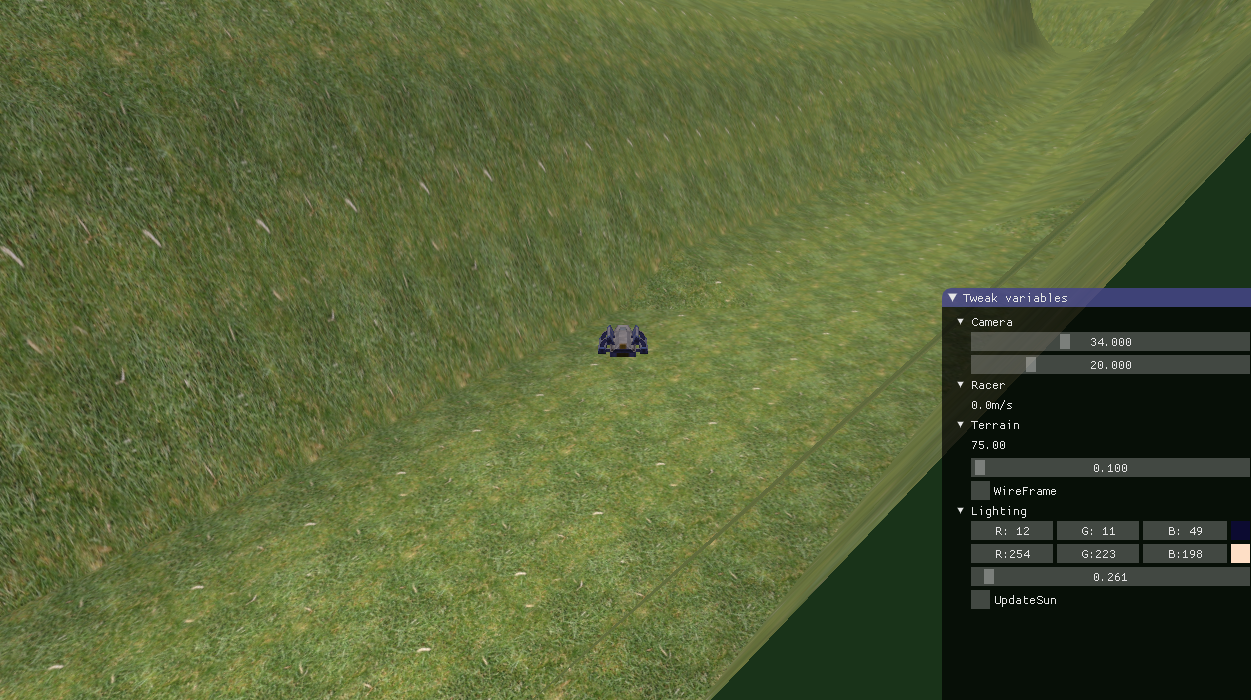
\includegraphics[scale=0.35]{/2_2.png}}
	\caption{Camera Rotating with the Racer}
	\label{fig:figure2}
\end{figure}
The result of rotating the camera can be seen in the above figure, please note that this screenshot was taken later into development of the game.

\section*{1.3 - Orientating and Placing the Racer Model}
This task for the racer required me to rotate and orientate the model. This model loading was very similar to the of Lab 1. To place the model at the racer's location I did the following:

\begin{lstlisting}  
        top = [0,0,1] # Define top in the Z-axis
        modelInWorld = lu.make_mat4_from_zAxis(self.position, self.heading, top)
        # Draw model in the specified world coordinates
        renderingSystem.drawObjModel(self.model, modelInWorld, view) 
\end{lstlisting}

First, I defined the top of the world in that of the z-axis. This was necessary as the task sheet recommended to do it and allowed me to use more functions. Using this top value, I made a 4x4 matrix using the racer's position, where it was heading and the top value defined earlier. Once I got this 4x4 matrix which represented coordinates to draw the model in, I then added the model to the coordinates and used the passed in view to place the Racer in the scene. 

\begin{lstlisting}  
	self.model = ObjModel(objModelName)
\end{lstlisting}

The last thing I did was load the model inside the racer's load function so the racer model could initialise on load. 

\begin{figure}[!ht]
	\centerline{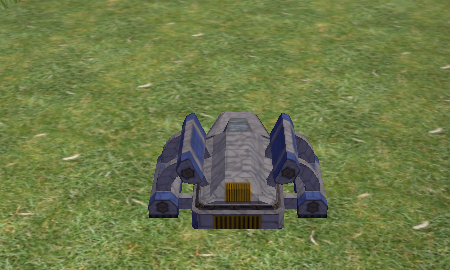
\includegraphics[scale=0.35]{/3_1.png}}
	\caption{The Loaded Model}
	\label{fig:figure3}
\end{figure}
Once loaded, I was able to rotate the model with the camera to allow for the racer model to always be facing forwards no matter which way the camera was adjusted to.

\section*{1.4 - Texturing the Terrain}
As you may have seen in previous figures, I was able to texture the terrain of the game.

\section*{1.5 - Lighting from the Sun}
- used shading solutions/what I learnt in lab 4
- noticed that the passed in values were:
vec3 materialColour, vec3 viewSpacePosition, vec3 viewSpaceNormal, vec3 viewSpaceLightPos, vec3 lightColour

did something similar
with global variable of globalAmbientLight

\end{document}

















